

\chapter{Elektronik}
Für die Elektronik ist Iterativ implementiert.
Anfangs wird mit einzelnen "Break out boards" gearbeitet. Diese sind einfach zu verbinden und können so relativ schnell zu einer funktionierenden Implementierung führen.

Diese haben jedoch das Risiko, dass das die Schaltungen sehr unübersichtlich werden. Daher wird im verlauf des Projektes eine Platine entwickelt. Das Kapitel zur ersten Implementierung ist im Anhang zu finden. Im weiteren wird die finale Bordelektronik beschrieben mit jeweiligen Anmerkungen und Verbesserungen.


\section{Grundanforderungen an die Elektronik}
Das Segelboot sollte über die nötigen mittel verfügen, eigenständig einen Kurs zu berechnen. Dafür wird ein Mikrocontroller benötigt.
Dieser muss mit Strom versorgt werden. Daher ist auch ein Energiesquelle notwendig. Um Autonomie zu gewährleisten muss diese durchgehend sein. Daher wird ein Energiepuffer bzw. eine Batterie benötigt. Der Gesamtenergieverbrauch des Bootes sollte im schnitt nicht mehr 0.8 W betragen. 

Damit der Mikrocontroller einen Kurs berechnen kann, müssen Umweltdaten bekannt sein. Diese sollen über Sensoren gemessen werden. Um den Kurs auch anzuwenden muss mit der Umwelt interagiert werden. Dafür sind Aktuatoren vorgesehen.






 \subsection{Grundaufbau der Platine}
Um eine übersichtliche Implementierung der Bordelektronik zu gewährleisten wurde eine Platine entwickelt.


\begin{figure}[H]
    \centering
    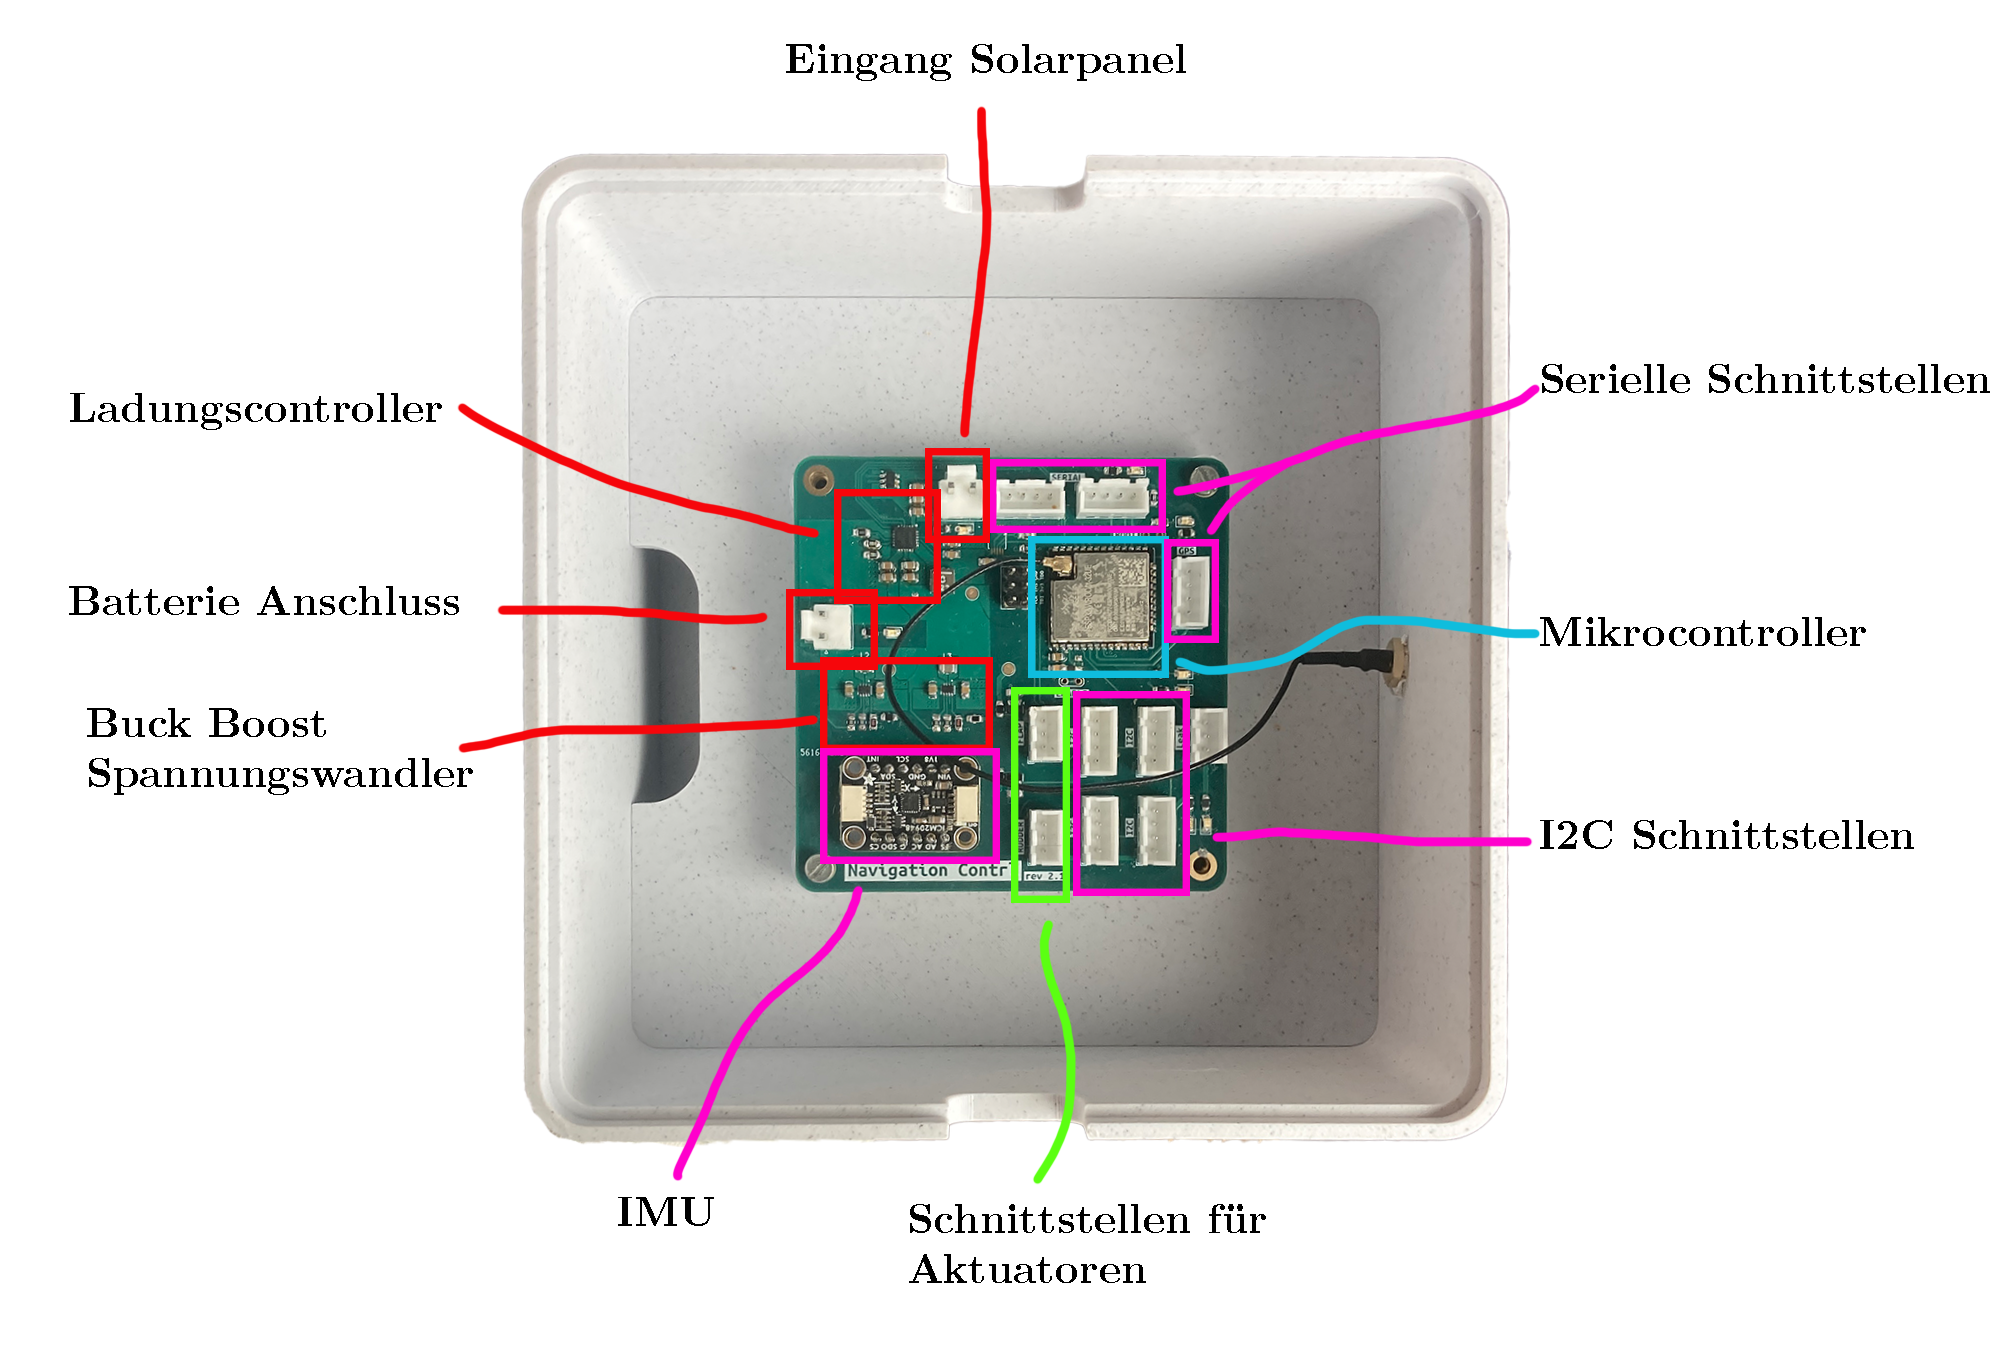
\includegraphics[width=1\linewidth]{Overview PCB_colored.png}
    \caption{Grundkomponenten der Platine}
    \label{fig:core_pcb}
\end{figure}
 
\begin{figure}[H]
    \centering
     \begin{subfigure}[b]{0.38\linewidth}
        \centering
        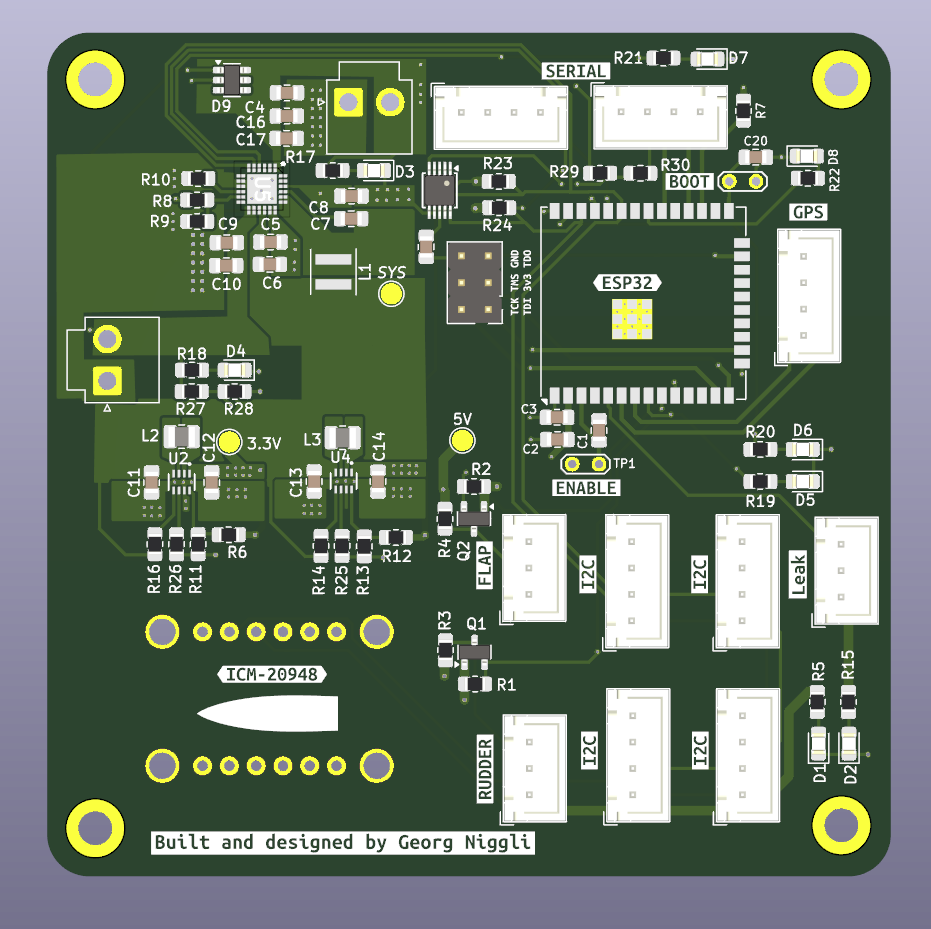
\includegraphics[width=\linewidth]{assets/pcb_2.png}
        \caption{Platine – Ansicht 3D}
        \label{fig:pcb_2}
    \end{subfigure}
    \hfill
      \begin{subfigure}[b]{0.38\linewidth}
        \centering
        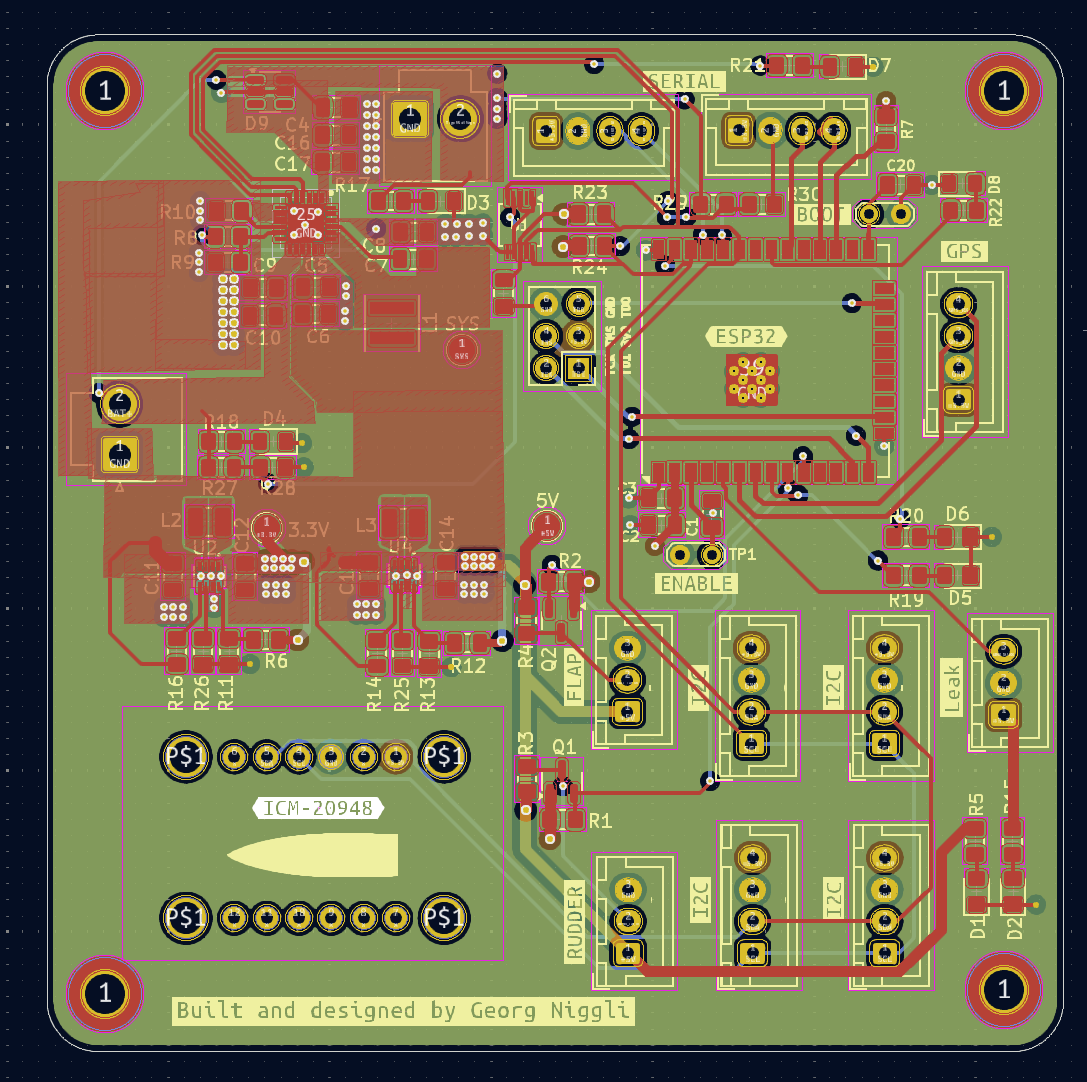
\includegraphics[width=\linewidth]{assets/pcb_1.png}
        \caption{Platine – Ansicht KiCad}
        \label{fig:pcb_1}
    \end{subfigure}
    \caption{Zwei Ansichten der entwickelten Leiterplatte}
    \label{fig:pcb_views}
\end{figure}


Die Grundkomponenten lassen sich wie in Abbildung \ref{fig:core_pcb} farblich dargestellt, in vier Kategorien aufteilen.
\begin{itemize}
    \item Mikrocontroller: Blau
    \item Energie und Leistungselektronik: Rot 
    \item Sensoren: Pink
    \item Aktuatoren: Grün 
\end{itemize}


\subsection{Mikrocontroller}

Ein ESP32-WROOM-32UE-N8R2 Modul von Espressif wird als Mikrocontroller verwendet. Module dieser Form werden aus einer zusätzlichen Platine hergestellt die alle essenziellen Funktionsschaltungen integriert haben. Somit könnend diese einfacher in neue Schaltungen integriert werden.\ref{ESP32Datasheet}

ESP32 Mikrocontroller sind sehr beliebt für ihre einfache Programmierung in der Arduino Umgebung. Zudem sind die Drahltloskommunikationsprotokolle WLAN und Bluetooth Low Energy (BLE) von Haus aus eingebaut. Im folgenden wird BLE verwendet.

Gewählt wird dieser Mikrocontroller aufgrund seiner relativ einfachen Programmierung im Vergleich zu anderen eingebetteten Systemen. Seine Rechenleistung reicht für die gewählte Implementierung des Navigationsalgorithmus aus. Der ESP32 ist nicht der Energiesparendste Mikrocontroller. Mit einem Energieverbrauch von 130 mA beim kommunizieren über Bluetooth Low Energy (BLE) liegt dies mit 0.4W noch deutlich unter der angepeilten Wattstunde und läst noch viel Raum übrig für die restlichen Bauteile.

Ein Raspberry Pi, der in der vorherigen Iteration verwendet wird, hat sich in der Implementierung als schwieriger dargestellt. Die Interaktion mit Sensoren über den eigentlich unterstützten I2C Bus hat nicht immer zuverlässig Funktioniert. Da die zusätzlichen Funktionen die eine Linux Umgebung bieten nicht benötigt werden, wird die einfachere und zuverlässigere Alternative gewählt.


\subsection{Batterieladung}
Zur geregelten Ladung des Akkumulators wird ein 5-A-Modul mit dem Lade-IC BQ25895 von Texas Instruments eingesetzt.  
Lithium-Ionen-Akkumulatoren dürfen nicht ausschliesslich mit konstantem Strom geladen werden. In Abbildung~\ref{fig:battery-curve} ist ein Diagramm aus dem Datenblatt des Lade-ICs dargestellt, das den typischen Verlauf eines Ladevorgangs zeigt. Dieses Ladeverfahren gewährleistet einen sicheren und Akkuschonenden Betrieb.

\subsubsection{Ladeprozess von Li-Ionen-Akkumulatoren}

\begin{figure}[H]
    \centering
    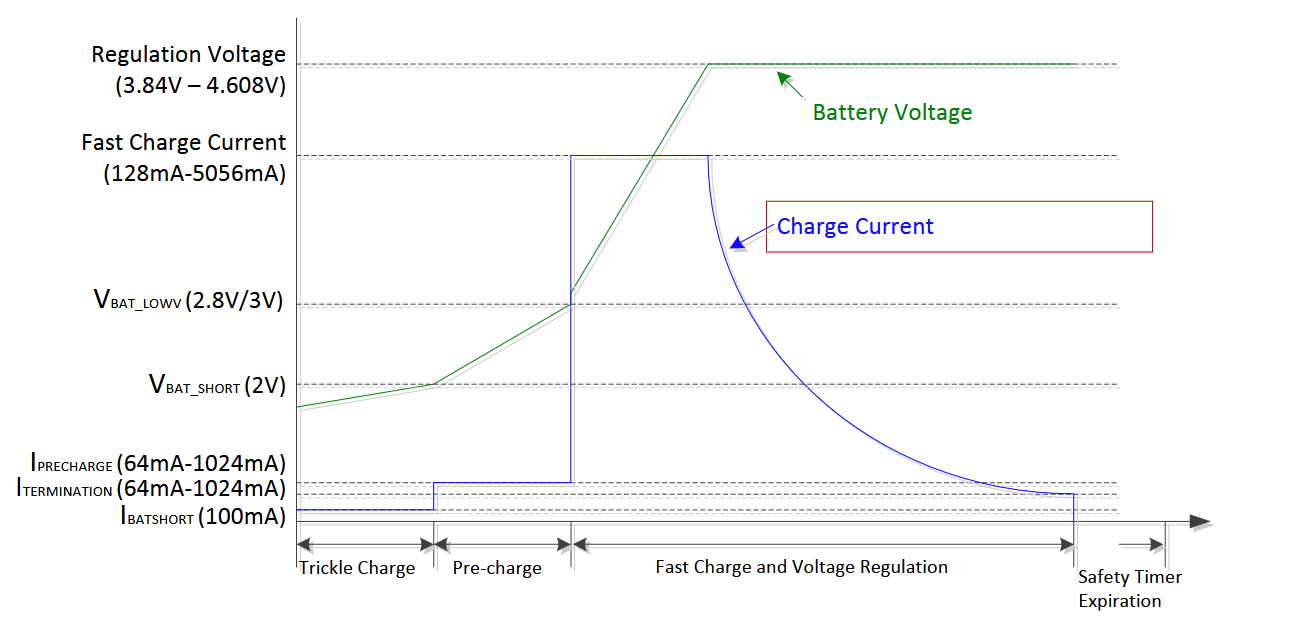
\includegraphics[width=0.7\linewidth]{batteryChargeCurve.png}
    \caption{Batterie Lade Kurve}
    \label{fig:battery-curve}
\end{figure}

Der Ladevorgang eines Lithium-Ionen-Akkumulators erfolgt in zwei Hauptphasen gemäss dem \textbf{CC-CV-Verfahren} (Constant Current – Constant Voltage):

\begin{itemize}
    \item \textbf{Konstantstromphase (CC):}  
    Zu Beginn des Ladevorgangs wird der Akku mit einem konstanten Strom geladen. Dabei steigt die Zellenspannung kontinuierlich an, bis sie den maximal zulässigen Wert erreicht (typischerweise 4{,}2\,V pro Zelle). Diese Phase dient dem schnellen Auffüllen der Zellkapazität und dauert etwa 60--70\,\% der gesamten Ladezeit.

    \item \textbf{Konstantspannungsphase (CV):}  
    Nach Erreichen der maximalen Zellspannung wird die Spannung konstant gehalten, während der Strom allmählich abnimmt. In dieser Phase erfolgt die vollständige Sättigung der Zelle mit Ladungsträgern.
\end{itemize}

Der Lade-IC BQ25895 erkennt das Ladeende automatisch anhand des sogenannten Terminationsstroms (\textit{I\_TERM}). Sobald der Ladestrom in der Konstantspannungsphase unter diesen Schwellwert fällt, beendet der IC den aktiven Ladevorgang. Der Terminationsstrom ist über das Register \texttt{CHARGE\_TERMINATION\_CURRENT} (Adresse \texttt{0x05}) konfigurierbar und beträgt standardmssig \textbf{180\,mA} 

Nach Erreichen dieses Punktes wechselt der IC in den Standby-Modus. Sollte die Zellenspannung später unter einen definierten Schwellenwert (typisch ca. 4{,}1\,V) fallen, wird der Ladevorgang automatisch erneut gestartet. Diese automatische Ladeende-Erkennung schützt den Akku vor Überladung.

Durch die Kombination der beiden Ladephasen sowie der intelligenten Ladeüberwachung wird eine sichere, vollständige und akkuschonende Ladung erreicht.


\subsection{Aufbau der Batterie}
Es ist vorgesehen, dass die Energiereserve einen Betrieb während zwei Tagen (48 h) erlauben soll. Der genaue Energieverbrauch des Rechners, der Sensoren und vor allem der Aktuatoren hängt stark davon ab, wie oft Steuereingriffe vorgenommen werden müssen und Messdatenerfassungen Neuberechnungen erfolgen. Es lässt sich daher nicht präzis berechnen, sondern nur abschätzen. 

Der Richtwert für den Gesamtenergieverbrauch pro Stunde beträgt maximal 0.8 Watt. Das ergibt einen Energieverbrauch von 19.2 Wattstunden pro Tag (24 h). Zur Überbrückung der vorgesehenen zwei Tagen ohne Energiezufuhr muss der Speicher daher über eine Kapazität von 38.4 Wattstunden verfügen. 

Eine völlige Erschöpfung des Energiespeichers kann diesen schädigen. Sie muss daher verhindert werden. Aber bereits ein Absinken der Ladung auf unter 20 Prozent verkürzt dessen Lebensdauer. Die Kapazität muss daher erhöht werden. Um über Reserven zu verfügen, wird daher eine Kapazität von 46.25 Wattstunden vorgesehen.

Für den Energiespeicher sollen 5 günstige wiederaufladbare EVE ICR18650 Litium-Ionen Zellen der chinesischen EVE Energy CO., LTD verwendet werden. Die Zellen haben eine Kapazität von 2'550 mAh un eine für Li-Ion übliche Nennspannung von 3.7 V.

\begin{figure}[H]
    \centering
    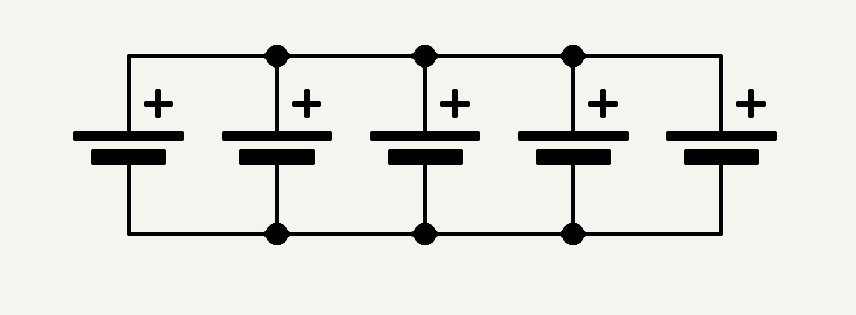
\includegraphics[width=0.5\linewidth]{assets/batterie_5p.png}
    \caption{Batterie 5 Parallel}
    \label{fig:bat5p}
\end{figure}

Es werden 5 Zellen parallel zusammengeschweisst. Hierfür wird ein übliches verfahren aus der Batterieherstellung verwendet. Das Punktschweissen. Es wäre an sich möglich, die Nikkelbänder mit denen die Zellen verbunden sind, zu verlöten. Dabei besteht aber die ernste Gefahr, dass die Zellen mit dem Lötkolben zu lange und zu stark erhitzt werden. Sie können dabei nicht nur unrettbar beschädigt werden, sondern sich auch entzünden.


Der Ladecontroller verfügt zudem über PowerPath was für die Anwendung in Autonomen Gefährten essenziell ist. PowerPath beschribt den Vorgang, bei dem das System durchgehend mit Enegerie versorgt wird. Auch dann, wenn die Batterie geladen wird. Somit kommt es zu keinen Unterbrüchen welche in dieser Anwendung verehrende Folgen haben könnten. 


\subsection{Energieversorgung}

Rechner, Sensoren und Aktuatoren werden mit elektrischer Energie betrieben. Weil das Segelboot autonom funktionieren soll, muss diese auf dem Schiff selbst gewonnen werden. Infrage kommen dabei grundsätzlich drei Energiequellen, nämlich Wasserenergie, Windenergie und Sonnenenergie.

\subsubsection{Wasserturbine}
Da sich das Boot im Wasser bewegt, könnte eine kleine Wasserturbine am Bootskörper befestigt und die Strömung zu deren Antrieb genutzt werden. Da sich das Boot relativ zum Wasser bewegt, gelten die gleichen Prinzipien wie bei Generierung elektrischer Energie durch Wasserkraft in Fliessgewässern.

Diese Methode hat jedoch gewichtige Nachteile. Segelboote erreichen, abgesehen von speziellen Konstruktionen wie sog. Foilingboote, bei denen der Bootskörper bei Fahrt vollständig aus dem Wasser gehoben wird, nur bescheidene Geschwindigkeiten. Da die Leistung einer Turbine in einer Flüssigkeit bei gleicher Fläche kubisch zur Strömungsgeschwindigkeit ansteigt, erlaubt diese Methode selbst bei idealen Segelbedingungen nur eine geringe Energieausbeute. Zudem würde das Segelboot durch die Turbine empfindlich abgebremst. 

\subsubsection{Windturbine}
Auch die Generierung von elektrischer Energie mithilfe einer Windturbine unter Nutzung der Windkraft ist nicht praktikabel. Um die Windenergie in Bewegungsenergie umzusetzen, aus der dann elektrische Energie generiert werden kann, muss ein Windrad in den Wind gedreht werden. Ein Segelboot kann keinen Kurs gegen den Wind segeln. Der Kurs vor dem Wind (also ein Kurs, bei dem der Wind von hinten auf das Boot trifft) ist zwar möglich, aber wenig effizient. Ein Windrad könnte folglich nicht fix mit dem Boot verbunden werden, sondern müsste drehbar ausgelegt werden, damit es unabhängig vom Kurs des Bootes in den Wind gedreht werden kann. Es müsste so platziert werden, dass nicht nur eine Berührung des Segels, sondern auch eine Berührung der Wasseroberfläche bei einer Kränkung (Schieflage) des Bootes ausgeschlossen ist. Damit müsste es am äussersten Bug, am äussersten Heck oder auf dem Mast platziert werden. Alle Positionen verbieten sich, da damit die Balance des Bootes akut gefährdet wäre. 

Schliesslich würde eine Positionierung am Bug oder Heck je nach vorherrschendem Wind, zu einer vollen oder teilweisen Abschattung des Windrades durch das Segel oder des Segels durch das Windrad führen. Eine Positionierung auf dem Mast würde selbst im Fall eines Vertikalwindrades zu Verwirbelungen führen, welche die Segeleigenschaften des Bootes negativ beeinträchtigen würden.

\subsubsection{Fotovoltaik}
Für die Nutzung der Sonnenenergie auf dem autonomen Segelboot kommt nur die Methode der Fotovoltaik infrage. Die für den Betrieb von Wärme-Kraft-Maschinen erforderlichen Temperaturen lassen sich auf einem beweglichen Boot mit Sonnenenergie nicht erreichen.

Die Energieerzeugung mit Fotovoltaikanlagen ist auf Segelbooten beliebt und verbreitet. Solche Anlagen haben keinen Einfluss auf die Segeleigenschaften des Bootes. Die Energieausbeute hängt aber stark vom Sonnenstand und dem vorherrschenden Wetter ab. Im Gegensatz zu stationären Anlagen lassen sich Fotovoltaikanlagen auf Booten nicht ideal auf die Sonne ausrichten und können je nach Kurs sogar vom Segel beschattet werden. Da während der Nachtstunden überhaupt keine Energie gewonnen werden kann, muss das Boot zur Überbrückung zwingend mit einem Energiespeicher ausgerüstet werden.

Das Solarpanel kann auf dem Deck oder am Festsegel befestigt werden. Die Befestigung auf dem Deck hat den Vorteil, dass die Verbindungsleitung zum Energiespeicher nicht durch den Schleifring geführt werden muss. Sodann ist die sichere Befestigung am flachen Deck einfacher als am gewölbten Festsegel. Schliesslich müssten bei einer Montage am Segel zwei Panels verwendet werden, damit beide Seiten des Festsegels damit ausgerüstet werden können. Andernfalls bestünde die Gefahr, dass sich das Panel bei einem ungünstigen Kurs längere Zeit auf der Schattenseite des Festsegels befindet.  

Der Selbstbau eines Panels wird nach einer längeren Erkundungsphase verworfen, da komplette, für den mobilen Einsatz entwickelte Panels kostengünstiger sind.   

Es wird das portable und faltbare Pi Juice Solar Panel - 22 Watt der britischen Pi Supply (Nebra Ltd) verwendet. Es ist gegen Spritzwasser geschützt (IP4X-Kennzeichnung), misst im entfalteten Zustand 83x23 cm und wiegt 520 g. Die vier einzelnen Panels sind von einer Textilhülle umfasst, die vier Befestigungsösen aufweist. Mit diesen wird das Panel vor dem Mast auf der flachen Deckplatte des Segelboots befestigt.

Bei den Solarzellen handelt es sich um monokristalline Siliziumzellen. Diese zeichnen sich durch einen hohen Wirkungsgrad sowie eine lange Lebensdauer aus und sind aufgrund ihrer gleichmässigen Kristallstruktur besonders effizient bei direkter Sonneneinstrahlung.

Ein wesentliches Problem bei der Verwendung von Solarzellen ist die Teilverschattung. Unter Teilverschattung versteht man die teilweise Abschattung einzelner Zellen oder Zellbereiche innerhalb eines Solarmoduls.

Das elektrische Verhalten von Solarzellen unter Teilverschattung ist nicht linear. Da Solarzellen innerhalb eines Moduls meist in Reihe geschaltet sind, bestimmt die am stärksten verschattete Zelle den Stromfluss im gesamten Strang. Wird eine einzelne Zelle teilweise verschattet, so sinkt deren Stromproduktion lokal erheblich. Aufgrund der Reihenschaltung wirkt die verschattete Zelle wie ein elektrischer Widerstand oder sogar als Last, was zu einem Leistungsabfall im gesamten Modul führen kann.

Da die Energieausbäute  des Solapanels jedoch genug sein sollte, kann auf Phasen mit weniger Ausbäute verzichtet werden.

Ebenfalls nicht implementiert ist ein Maximum Power Point Tracking (MPPT) jedoch verfügt der Batterieladungscontroller über Input Current Optimizer (ICO)

\textbf{Unterschied zwischen ICO und MPPT:}
Der ICO und das MPPT sind zwei unterschiedliche Verfahren zur Leistungsoptimierung bei Energiequellen wie Solarpanels. Während MPPT darauf abzielt, den Arbeitspunkt des Panels so zu regeln, dass die abgegebene Leistung (Produkt aus Spannung und Strom) maximal ist, konzentriert sich ICO auf die Optimierung des Eingangsstroms. MPPT ist komplexer, reagiert dynamisch auf Umweltbedingungen und wird meist in grösseren Solaranlagen eingesetzt. ICO hingegen wird typischerweise in integrierten Power-Management-ICs verwendet, wie dem verwendeten BQ25895, und bietet eine einfachere Möglichkeit, die Quelle vor Überlastung zu schützen, indem es den optimalen Eingangsstrom einstellt.


Die maximale regulierte Ausgangsleistung beträgt 20 W bei 5 V. Es verfügt über zwei 5 V/ 2.4 A USB Ausgänge, wobei die maximale Ausgangsleistung pro USB Buchse auf 12 W beschränkt ist. Die zwei USB Buchsen können simultan benutzt werden.
\begin{figure}[H]
\centering
    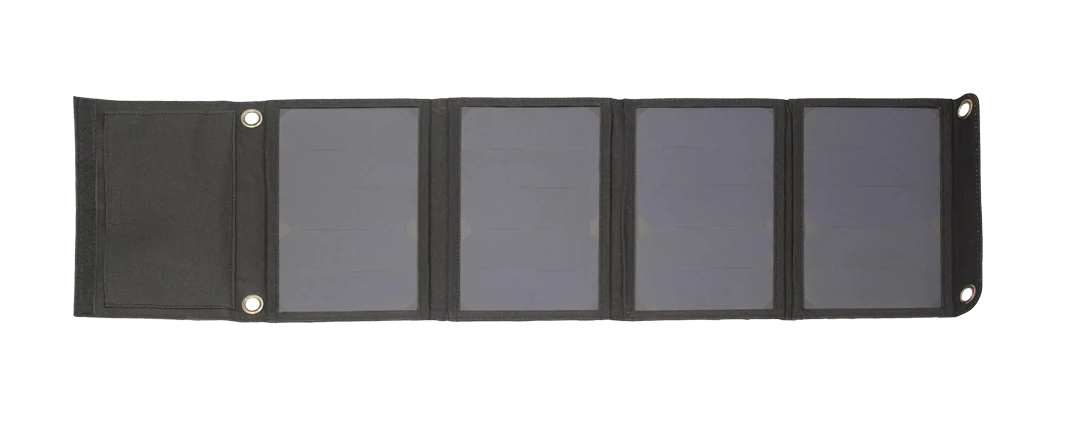
\includegraphics[width=1\linewidth]{assets/Pi juce.png}
    \caption{Pi Juce Solarpanel}
    \label{fig:enter-label}
\end{figure}

\subsection{Leistungselektronik}
Da sich auf dem Boot verschiedene Spannungen befinden, sind Spannungswandler notwendig. Der Mikrocontroller und alle Sensoren benötigen 3.3 V. Die Aktuatoren zur Steuerung des Ruders und des Segels benötigen 5V. Das Solarpanel hat eine Spannung von 5V und die Batterie eine Nennspannung von 3.7. Dieser Wert kann jedoch zwischen 3.3 V und 4.2 V variieren. Abhängig von der Ladung der Batterie.

Um nun geregelte Spannungen zu erzeugen werden zwei Buck Boost Konverter verwendet. 

Ein Buck-Boost-Konverter ist eine Gleichspannungswandler-Schaltung, die eine Eingangsspannung \( V_{\text{in}} \) in eine Ausgangsspannung \( V_{\text{out}} \) umwandelt, die entweder grösser oder kleiner als die Eingangsspannung sein kann. 

Der Buck Boost wurde hier im Gegensatz zum Regulären Buck Konverter gewählt, da die Batteriespannung sehr nahe oder sogar unterhalb von den benötigten 3.3 V liegen kann. Es ist essenziell, das dass System auch dann weiter funktioniert.

Verwendet werden zwei TPS631000DRLR vom Unternehmen Texas Instruments. Beide haben eine Effizienz von $\approx$ 90\%.

Die Schaltung ist der "Typical Application" aus dem Datenblatt nachempfunden.
\section{Sensoren und Aktuatoren}
\subsubsection{Positionsbestimmung (GPS)}
Zur Positionsbestimmung, also der Bestimmung des aktuellen Standorts des Segelboots, werden Funksignale des bekannten US-amerikanischen satellitenbasierten Global Positioning Systems (GPS) (deutsch Globales Positionsbestimmungssystem) offiziell NAVSTAR GPS verwendet. Dafür wird das Empfängermodul Whadda Neo 7M der belgischen Velleman Group nv verwendet, welches alternativ Signale des entsprechenden russischen Systems GLONASS empfangen kann.
Das Modul wird wie allen anderen sensoren über JST Stecker mit dem PCB verdrahtet und kommuniziert über eine serielle Verbindung. Das Modul wird mit 3.3 V betrieben.
\begin{figure}[H]
    \centering
    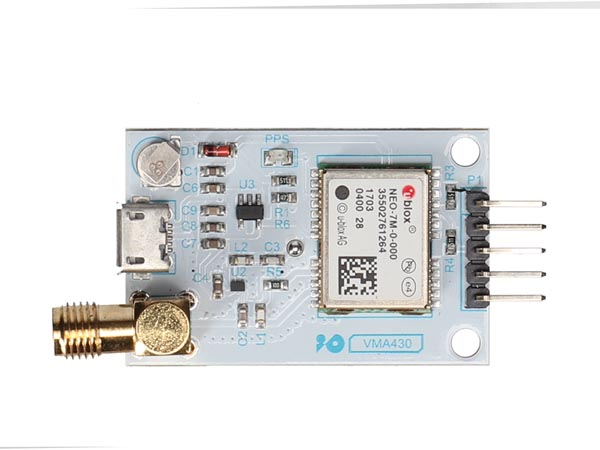
\includegraphics[width=0.75\linewidth]{vma430_front-1.jpg}
    \caption{GPS Modul - Oberseite}
    \label{fig:enter-label}
\end{figure}
Das Modul wird auf dem Deck im des Bootes platziert. Weil das Kunststoffgehäuse sehr dünn ist, kann auf eine externe Empfangsantenne verzichtet werden. Die vorhandene SMA Antennen Steckbuchse bleibt damit unbenutzt. Es wird die eingebaute keramische Patchantenne verwendet. In der unten stehenden Abbildung \ref{fig:GPS} ist diese als rosa Fläche mit einem metallenen Knopf auf einem beigen Körper sichtbar.
\begin{figure}[H]
    \centering
    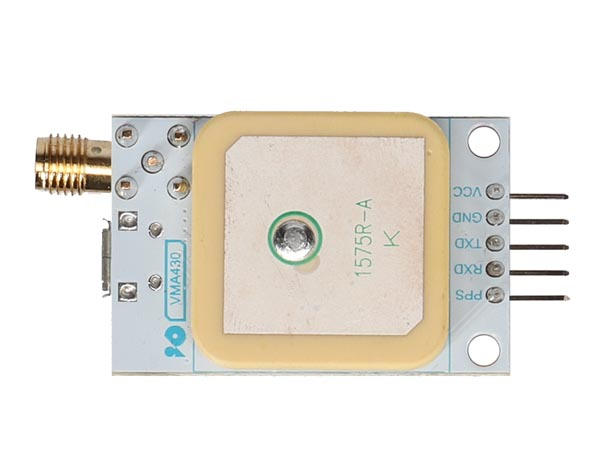
\includegraphics[width=0.5\linewidth]{vma430_back-1.jpg}
    \caption{GPS Modul}
    \label{fig:GPS}
\end{figure}

\subsubsection{Gyro und Magnetometer}

Zur Bestimmung der Richtung des Segelboots dient ein Magnetometer. Ein Magnetometer ist eine sensorische Einrichtung zur Messung magnetischer Flussdichten \cite{noauthor_magnetometer_2023}. Im vorliegenden Projekt wird das Magnetometer dafür eingesetzt, um damit einen Magnetkompass zu realisieren, indem das erdmagnetische Feld dreidimensional erfasst wird, um daraus die Bootsrichtung abzuleiten. Dieses Verfahren wird auch in Smartphones zur Richtungsbestimmung angewendet.

Im vorliegenden Projekt wird dafür das Sensormodul ICM-20948 der Firma Adafruit vorgesehen. Das Modul ist zusätzlich mit einem Gyroskop und einen Beschleunigungsmesser ausgestattet. Auch damit kann die Bewegung des Segelbootes erfasst werden. Ausserdem erlaubt es die Bestimmung der Schräglage des Segelbootes. Im vorliegenden Projekt wird dieser Wert erfasst jedoch nicht ausgewertet.

Das Sensormodul wird mit einer Eingangsspannung von 3.3 V betrieben und über den im PCB verbauten I2C Bus angehängt.



\section{Eigenentwicklung des Windrichtungssensors}
Der Windrichtungssensor muss selbst entwickelt und gebaut werden, da die am Markt angebotenen Windrichtungsmesser entweder zu gross und zu schwer oder unerschwinglich teuer sind.

Windrichtungssensoren lassen sich in zwei unterschiedliche Typen einteilen. Der erste Typ verwendet ein Potenziometer zur Richtungsbestimmung. Solche Messgeräte sind mechanisch sehr leicht umzusetzen, da dazu lediglich ein kleiner Flügel an der Achse eines Potenziometers befestigt werden muss. Die Position des Flügels kann damit über einen analogen Input Pin mit einem Mikrocontroller eingelesen und daraus die Richtung des Windes abgeleitete werden. Der Nachteil dieses Typs ist, dass die freie Drehung der Achse durch die Reibung das Potenziometers stark abgebremst wird. Dieser Typ wird daher nicht weiter verfolgt.

Der andere Typ verwendet Hallsensoren, welche den Hall-Effekt zur Messung von 
Magnetfeldern nutzen \cite{noauthor_hall-sensor_2023}. Sie sind passive Sensoren, die den Spannungsunterschied messen, der an einem elektrischen Leiter erzeugt wird, wenn ein Magnetfeld senkrecht zur Fliessrichtung eines elektrischen Stroms steht \cite{noauthor_alles_nodate}. Um die Rotation eines Objektes mittels Hallsensoren zu messen, gibt es die folgenden zwei Möglichkeiten:

Bei der ersten Variante wird um ein abwechselnd magnetisch positiv und magnetisch negativ geladenes rundes Objekt mehrere Hallsensoren platziert. Damit kann dann die Drehung des Objektes gemessen werden. Diese Variante ist praktisch schwierig umzusetzen, weil viele Hall Sensoren präzis kreisförmig um eine Achse angeordnet werden müssen. Diese Variante ist jedoch sehr umständlich im Vergleich zur zweiten Variante.

Die zweite Variante ist praktisch einfacher umzusetzen. Statt normale Hall Sensoren werden dabei spezielle, sogenannten Rotary Hall (deutsch rotierende magnetische Hall) Encoder verwendet. Ein Encoder (oder Messwertgeber) dient in der Antriebstechnik zur Signalbildung aus mechanischen Bewegungen. Er erkennt die Position einer Antriebseinheit (Welle) und gibt diese als elektrisches Signal aus. \cite{noauthor_was_nodate} Rotary Hall Encoder sind komplexe Bauteile, die fast immer als System-on-Chip gefertigt, in dem integrierte Hall-Elemente, analoges Frontend und digitale Signalverarbeitung in einem einzigen Gerät integriert sind. Zur Messung des Winkels wird nur ein einfacher zweipoliger Magnet benötigt, der sich der sich über oder unter der Mitte des Chips dreht.

Zur Funktionsweise von Rotary Hall Encodern: Josef Janisch, Understanding Integrated Hall Effect Rotary Encoders, Nov 1, 2006 1:00am, auf Fierce Electonics \cite{janisch_understanding_2006}.

Für das vorliegende Projekt wird ein Windsensor auf der Basis eines Rotary-Hall-Encoders vorgezogen. Dabei wird der auf einem Adapterboard gelötete AS5600 der österreichischen ams-OSRAM AG verwendet. Das ist ein berührungsloser Rotary Hall Encoder für genaue Winkelmessung über eine volle Umdrehung von 360$^\circ$.  Die absolute Winkelmessung liefert eine sofortige Anzeige der Winkelposition des Magneten mit einer Auflösung von 0.0879$^\circ$ = 4096 Positionen pro Umdrehung. Diese digitalen Daten stehen als I2C Bus zur Verfügung. Für das vorliegende Projekt wird der Sensor an den allgemeinen I2C bus der Platine angeschlossen. Somit kann die absolute position abgelesen werden. 

Der Encoder kann mit 3,3 V oder 5 V betrieben werden. Quellen für beide Spannungen sind auf dem Segelboot vorhanden. Da er I2C Bus aber auf 3.3V basiert wird auch dies zum betrieb des Rotary encoders verwendet.

Die restlichen Teile des Windrichtungssensors werden von Grund auf selbst entworfen und gebaut. Es handelt sich dabei um die Bodenplatte, das Gehäuse, die Welle und den Windflügel. Die vier Teile wurden mit dem CAD Programm entworfen und mit dem 3D Drucker gedruckt.

Der drehbare Windflügel verfügt am Ende über ein Segel, damit er sich selbständig in den Wind dreht. Er ist 15 cm lang.
\begin{figure}[H]
    \centering
    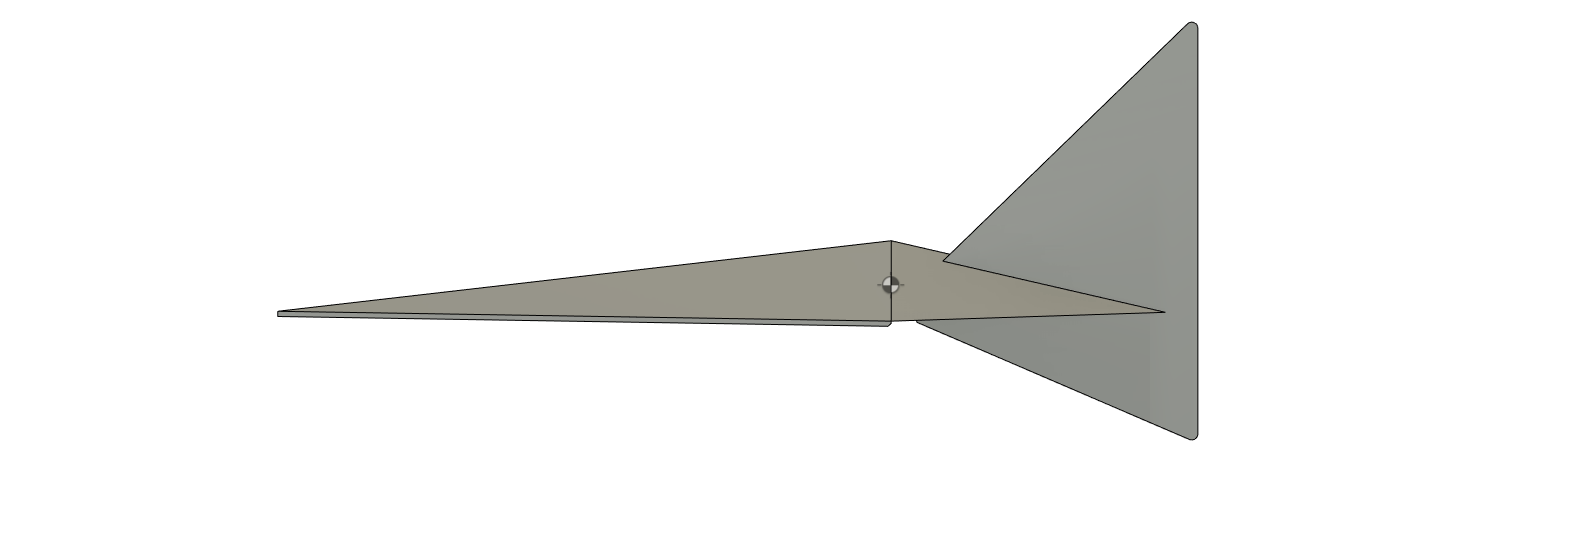
\includegraphics[width=0.75\linewidth]{assets/windsensor_top.png}
    \caption{Windflügel}
    
\end{figure}

Der Windflügel wird fest mit der Welle verbunden. Diese wird dann von oben ins leere Gehäuse geführt. Das Gehäuse weist dafür eine Öffnung auf, in welcher ein Kugellager verleimt wird, damit sich die Welle frei drehen kann. Die Konstruktion ist so ausgelegt, dass der Massemittelpunkt unabhängig von der Lage des Segelboots genau auf dem Drehpunkt des Windflügels liegt. Damit ist sichergestellt, dass auch bei den häufigen Schräglagen korrekte Werte ermittelt werden.

Das Gehäuse steht auf einer am Deck des Segelbootes gefestigten Grundplatte. Es hebt den Windflügel in den Wind und schützt die Adapterplatte mit dem Rotary-Hall-Encoder vor der Witterung und Wellen.


Der Windrichtungssensor wird an der Spitze des Bootes mit der Deckplatte verklebt.
\begin{figure}[H]
    \centering
    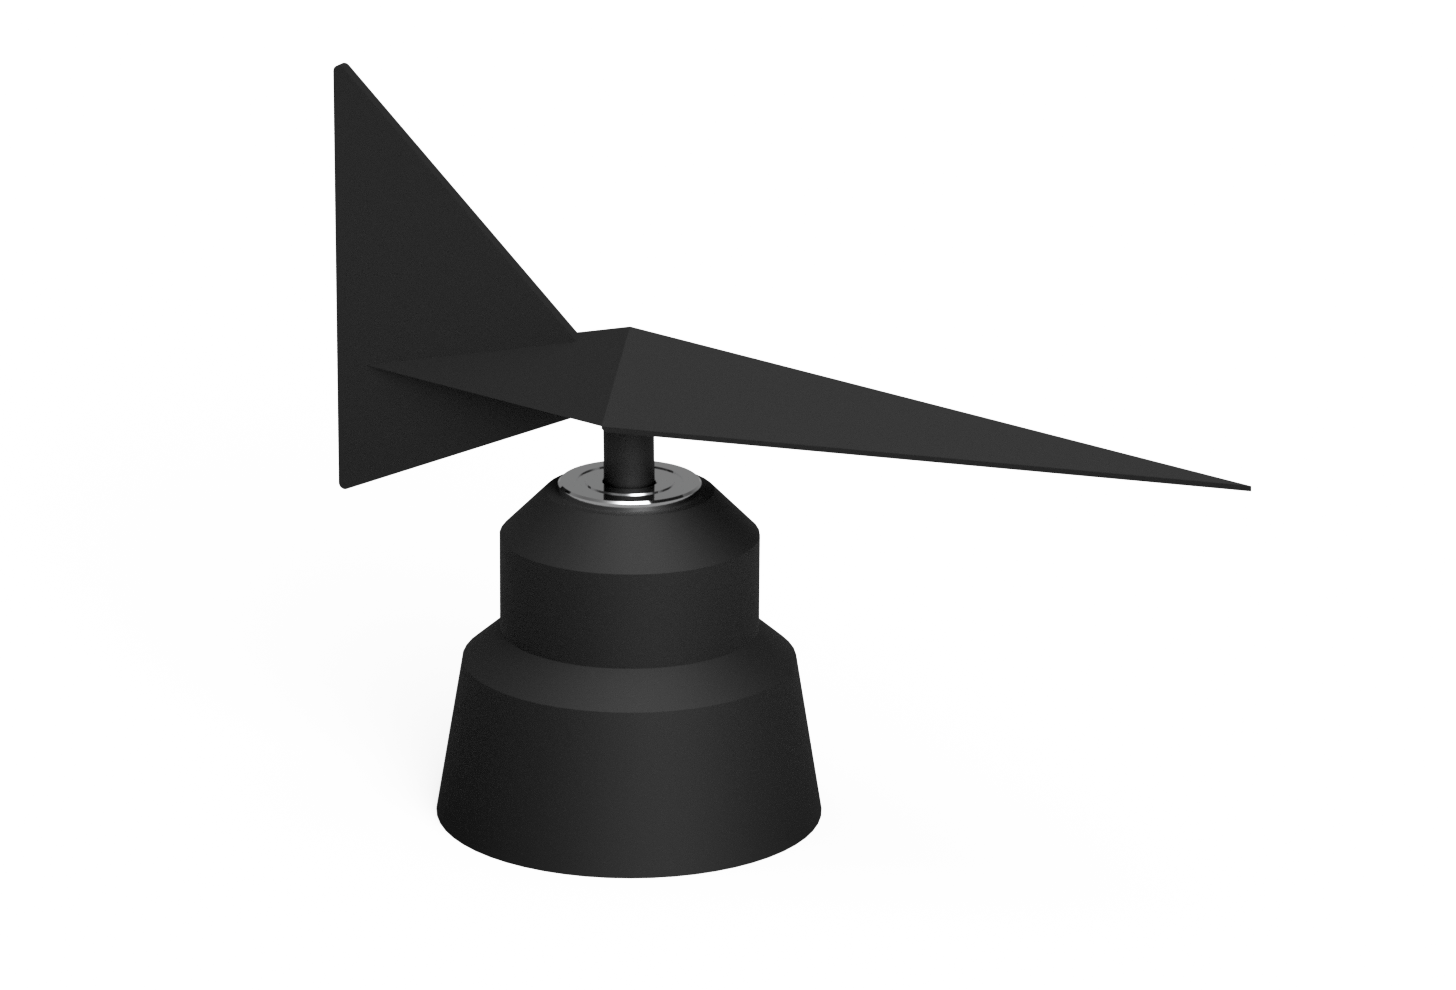
\includegraphics[width=0.75\linewidth]{assets/full_wind_sensor.png}
    \caption{Kompletter Windrichtungssensor}
    \label{fig:enter-label}
\end{figure}

\subsubsection{Aktuatoren}
Für die Bewegung des Ruders und des Sailflaps werden Aktuatoren verwendet. Aktuatoren (auch als Aktoren bezeichnet) sind das signalwandlerbezogene Gegenstück zu Sensoren. Sie setzen bei einem Bewegungsregelungsvorgang Signale durch mechanische Arbeit in Wirkungen um \cite{noauthor_aktor_2023}. Zur Bewegung von Ruder und Sailflaps werden elektrische lineare Aktuatoren benötigt. Ein elektrischer Linearantrieb ist ein Gerät, das die Drehbewegung eines Wechsel- oder Gleichstrommotors in eine lineare Bewegung umwandelt. Er kann sowohl Schub- als auch Zugbewegungen ausführen.

Für das vorliegende Projekt werden zwei L16-100-63-6 Serie R Aktuator der kanadischen Actuonix Motion Devices Inc. verwendet. Diese sind für den Einsatz in der Robotik und im Modellbau entwickelt worden und wasserdicht. Damit sind sie für den Einsatz auf Segelbooten prädestiniert.

Die Aktuatorwelle aus Aluminium verfügt über einem Maximalhub von 100 mm. Die Maximalgeschwindigkeit liegt ohne Last bei 20 mm/s. Damit sind sie nicht besonders schnell, verfügen mit 100N Stoss- und 46N Zugkraft aber über ausreichende Kraft zur Bewegung von Ruder und Sailflaps. Ihr Peak Power Point (der spezifische Geschwindigkeits- und Kraftpunkt, an dem die grösste Leistungsabgabe erfolgt) liegt bei 75N bei 10 mm/s. Das Getriebe der Aktuatoren weist eine Übersetzung von 63:1 auf.

\begin{figure}
    \centering
    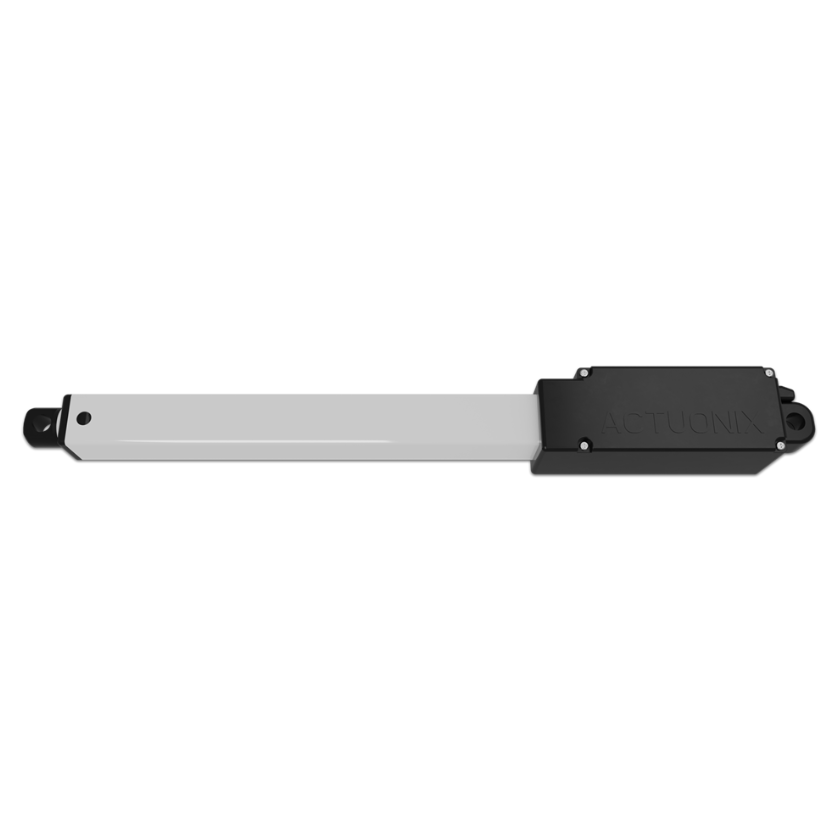
\includegraphics[width=0.75\linewidth]{actuonix.png}
    \caption{Actuonix Aktuator}
    \label{fig:actuator}
\end{figure}

Die Aktuatoren verfügen über kein digitales Positionsfeedback, das heisst, dass nicht abgefragt werden kann, an welcher Position sich das Ende der ausfahrbaren Welle befindet. Es können jedoch konkrete Distanzen angesteuert werden. 

Über eine einzige Datenleitung können kurze Impulse zwischen 1ms-2ms gesendet werden, wobei 1ms den Aktuator in die Startposition führt und der Aktuator bei 2ms voll ausgefahren wird. Um Einstellungen dazwischen zu erhalten, wird ein Wert zwischen 1ms und 2ms gesendet. 

Die Steuerleitung des Aktuators kann nicht direkt mit dem ESP32 verbunden werden, da dieser an seinen Pins nur 3,3 V Steuersignale ausgibt, der Aktuator aber ein 5 V Steuersignal erwartet. Aus diesem Grund muss zwischen den beiden Aktuatoren und dem ESP32 ein einfacher Pegelumsetzer (lever shifter) geschaltet werden. 
\begin{figure}[H]
    \centering
    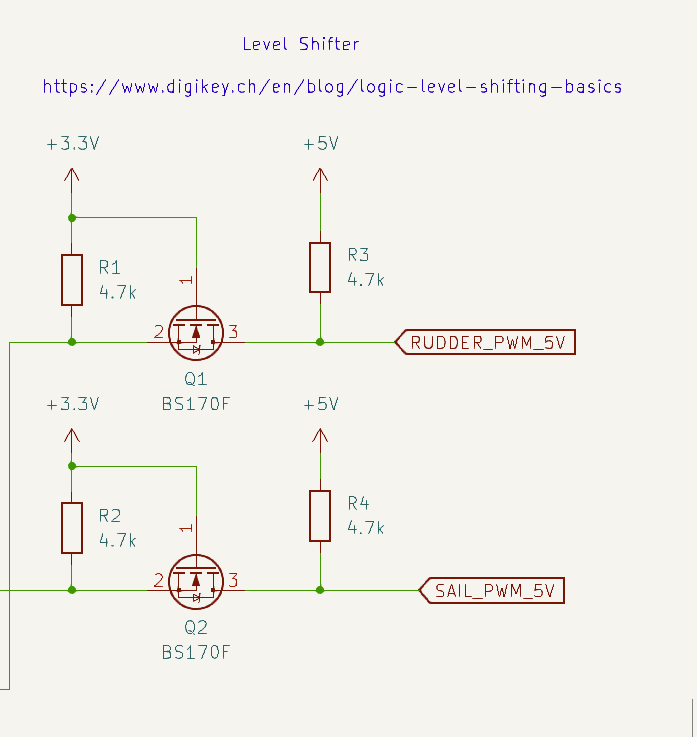
\includegraphics[width=0.5\linewidth]{assets/lvelshift.png}
    \caption{Schaltung Level Shifter von Sparkfun}
    \label{fig:enter-label}
\end{figure}

\subsection{Schleifring (Slip Ring)}
Der Aktuator zur Bewegung der Sailflaps muss an der Platine verkabelt sein. Da das Segel frei rotiert und sich um die eigene Achse drehen kann, besteht die Gefahr, dass die Verbindungskabel um den Mast gewickelt werden und reissen.

Dieser Gefahr kann mit dem Einsatz eines sogenannten Schleifrings begegnet werden.  Ein Schliefring ist ein elektromechanisches Bauteil, das eine elektrische Leistungs- oder Signalübertragung zwischen gegeneinander rotierenden Bauteilen ermöglicht. Er besteht aus einem stromleitenden Ring und Bürsten, die in Kontakt mit diesem Ring stehen. Die Bürsten bestehen aus einem leitfähigen Material und sind mit der stationären Struktur des Systems verbunden. 

Der Schleifring wird am Fuss des Segelmastes montiert und mit dem Schiffskörper verschraubt. Durch den hohlen Mast werden dann die drei Leistungen hinauf zum Segel gezogen und durch ein in den Mast gebohrtes Loch zum Aktuator geführt und mit diesem verbunden.

















